\documentclass[a4paper,12pt]{article}
\usepackage{float} %здесь здесь, только здесь
%%% Работа с русским языком
\usepackage{cmap}					% поиск в PDF
\usepackage{mathtext} 				% русские буквы в формулах
\usepackage[T2A]{fontenc}			% кодировка
\usepackage[utf8]{inputenc}			% кодировка исходного текста
\usepackage[english,russian]{babel}	% локализация и переносы

%%% Дополнительная работа с математикой
\usepackage{amsmath,amsfonts,amssymb,amsthm,mathtools} % AMS
\usepackage{icomma} % "Умная" запятая: $0,2$ --- число, $0, 2$ --- перечисление

%% Номера формул
%\mathtoolsset{showonlyrefs=true} % Показывать номера только у тех формул, на которые есть \eqref{} в тексте.
%\usepackage{leqno} % Нумерация формул слева

%% Свои команды
\DeclareMathOperator{\sgn}{\mathop{sgn}}

%% Перенос знаков в формулах (по Львовскому)
\newcommand*{\hm}[1]{#1\nobreak\discretionary{}
	{\hbox{$\mathsurround=0pt #1$}}{}}

%%% Работа с картинками
\usepackage{graphicx}  % Для вставки рисунков
\graphicspath{{images/}{images2/}}  % папки с картинками
\setlength\fboxsep{3pt} % Отступ рамки \fbox{} от рисунка
\setlength\fboxrule{1pt} % Толщина линий рамки \fbox{}
\usepackage{wrapfig} % Обтекание рисунков текстом

%%% Работа с таблицами
\usepackage{array,tabularx,tabulary,booktabs} % Дополнительная работа с таблицами
\usepackage{longtable}  % Длинные таблицы
\usepackage{multirow} % Слияние строк в таблице

%%% Теоремы
\theoremstyle{plain} % Это стиль по умолчанию, его можно не переопределять.
\newtheorem{theorem}{Теорема}[section]
\newtheorem{proposition}[theorem]{Утверждение}

\theoremstyle{definition} % "Определение"
\newtheorem{corollary}{Следствие}[theorem]
\newtheorem{problem}{Задача}[section]

\theoremstyle{remark} % "Примечание"
\newtheorem*{nonum}{Решение}

%%% Программирование
\usepackage{etoolbox} % логические операторы

%%% Страница
\usepackage{extsizes} % Возможность сделать 14-й шрифт
\usepackage{geometry} % Простой способ задавать поля
\geometry{top=25mm}
\geometry{bottom=35mm}
\geometry{left=35mm}
\geometry{right=20mm}
%

\usepackage{fancyhdr} % Колонтитулы
\pagestyle{fancy}
\renewcommand{\sectionmark}[1]{\markboth{#1}{}}
%\renewcommand{\headrulewidth}{0mm}  % Толщина линейки, отчеркивающей верхний колонтитул
%\lfoot{Нижний левый}
%\rfoot{Нижний правый}
%\rhead{}
%\chead{Верхний в центре}
\lhead{\thepage}
\cfoot{} % По умолчанию здесь номер страницы

\usepackage{setspace} % Интерлиньяж
%\onehalfspacing % Интерлиньяж 1.5
%\doublespacing % Интерлиньяж 2
%\singlespacing % Интерлиньяж 1

\usepackage{lastpage} % Узнать, сколько всего страниц в документе.

\usepackage{soul} % Модификаторы начертания

\usepackage{indentfirst} % Красная строка

\usepackage{soulutf8} % Модификаторы начертания

%\usepackage{hyperref}
%\usepackage[usenames,dvipsnames,svgnames,table,rgb]{xcolor}
%\hypersetup{				% Гиперссылки
%	unicode=true,           % русские буквы в раздела PDF
%	pdftitle={Заголовок},   % Заголовок
%	pdfsubject={Тема},      % Тема
%	pdfcreator={Создатель}, % Создатель
%	pdfproducer={Производитель}, % Производитель
%	pdfkeywords={keyword1} {key2} {key3}, % Ключевые слова
%	colorlinks=true,       	% false: ссылки в рамках; true: цветные ссылки
%	linkcolor=red,          % внутренние ссылки
%	citecolor=green,        % на библиографию
%	filecolor=magenta,      % на файлы
%	urlcolor=cyan           % на URL
%}

%\renewcommand{\familydefault}{\sfdefault} % Начертание шрифта

% объявляем новую команду для переноса строки внутри ячейки таблицы
\newcommand{\specialcell}[2][c]{%
	\begin{tabular}[#1]{@{}c@{}}#2\end{tabular}}

\usepackage{multicol} % Несколько колонок

\author{\LaTeX{} в Вышке}
\title{3.2 Оформление документа в целом}
\date{\today}

\begin{document} % конец преамбулы, начало документа
	\thispagestyle{empty}
	\begin{center}
		\textit{Федеральное государственное автономное образовательное\\ учреждение высшего образования }
		\vspace{0.5ex}
		
		\textbf{«Московский физико-технический институт\\ (национальный исследовательский университет)»}
	\end{center}
	\vspace{10ex}
	%\begin{flushright}
	%	\noindent
	%	\textit{Фамилия Имя Отчество}
	%	\\
	%	\textit{студент факультета экономики \\(группа 211И)}
	%\end{flushright}
	\begin{center}
		\vspace{13ex}
		\so{\textbf{Лабораторная работа №2.1.2}}
		\vspace{1ex}
		
		по курсу общей физики
		
		
		на тему:
		
		\textbf{\textit{<<Определение $C_p/C_v$ методом \\ адиабатического расширения газа>>}}
		\vspace{30ex}
		\begin{flushright}
			\noindent
			\textit{Работу выполнил:}
			\\
			\textit{Баринов Леонид \\(группа Б02-827)}
		\end{flushright}
		\vfill
		Долгопрудный \\2019
	\end{center}
	\newpage
	\setcounter{page}{1}
	\section{Аннотация}
	В работе будет измерен показатель адиабаты  для воздуха $\gamma = C_p/C_v$ методом Клемана-Дезорма.
	\section {Теоретические сведения}
	\subsection{Адиабатический процесс}
	Процесс, происходящий без теплообмена с окружающей средой, называется адиабатическим. Получим уравнение такого процесса для идеального газа, внутренняя энергия которого $U$ не зависит от объёма.
	
	Из первого начала термодинамики при $\delta Q = 0$ для идеального газа, у которого $dU = C_v dT$, получим $C_v dT + P dV = 0$. Исключим отсюда давление $P$ c помощью уравнения состояния $pV = RT$:
	\[C_V\frac{dT}{T}+R\frac{dV}{V} = 0 \]
	
	При постоянной величине $C_v$, что соответствует классической теории теплоемкости, уравнение легко интегрируется:
	\[TV^{R/C_v} = TV^{\gamma - 1} = \text{const} \]
	
	Это уравнение адиабатического процесса в переменных $T, V$. Преобразуем его к переменным $p, V$. Снова используя $pV = RT$, а также соотношение Майера, получим уравнение, которое называется также адиабатой Пуассона:
	\begin{equation}
	pV^{\gamma} = \text{const}
	\end{equation}
	Здесь $\gamma$ -- показатель адиабаты.
	\begin{equation}
	\gamma = \frac{C_p}{C_v}
	\end{equation}
	
	\subsection{Измеримые величины}
	Используя уравнения состояния идеального газа перепишем уравнение (1) в виде:
	\begin{equation}
	pT^{\gamma/(1-\gamma)} = \text{const}
	\end{equation}
	Возьмем от выражения (3) производную. Получим:
	\[\frac{dT}{T} = \frac{\gamma - 1}{\gamma}\frac {dp}{p} \]
	Перейдем к конечным приращениям. $\Delta p \ll p_0$, где $p_0$ - атмосферное давление:
	\begin{equation}
	\frac{\Delta T}{T} = \frac{\gamma - 1}{\gamma}\frac {\Delta p}{p}
	\end{equation}
	Из формулы (4) следует, что при малых перепадах давления, порядка нескольких кПа, достаточно точно измеряемых водяным манометром, снижение температуры при адиабатическом расширении оказывается малым, порядка одного Кельвина.
	
	Что бы определить понижение температуры $\Delta T$ в адиабатическом процессе, в методе Клемана-Дезорма используется последующий вспомогательный процесс изохорного нагрева до исходной комнатной температуры, и величина  $\Delta T$ рассчитывается по росту давления газа в ходе этого процессе. Таким образом, рабочий газ используется в качестве газового термометра
	
	\section{Оборудование}
	В работе используются: стеклянный сосуд; $U$--образный жидкостный манометр; резиновая груша; газгольдер с углекислым газом.
	\subsection{Экспериментальная установка}
	Используемая для опытов установка состоит из стеклянного сосуда $\text{А}$ (объемом около 20 л), снабженного краном $\text{К}$, и $U$--образного жидкостного манометра, измеряющего избыточное давление газа в сосуде. Схема установки показана на рисунке 1.
	
	Избыточное давление воздуха создается с помощью резиновой груши, соединенной с сосудом трубкой с краном $\text{К}_1$. 
	\begin{figure}[H]
		\begin{center}
			\includegraphics[width=0.7\linewidth]{1}
			\caption{Установка для определения $C_p/C_v$ методом адиабатического расширения газа}
		\end{center}
	\end{figure}
\subsection{Последовательность проводимых термодинамических процессов}
Последовательность представлена на Рис. 2. Обозначим через $p_0, V_0, T_0$ исходные параметры рабочей порции газа ($p_0, T_0$ -- давление и температура окружающей атмосферы)
\begin{figure}[H]
	\begin{center}
		\includegraphics[width=0.7\linewidth]{2}
		\caption{$p-V$ - диаграмма процессов в газе}
	\end{center}
\end{figure}
\begin{itemize}
	\item $1\rightarrow2$ \\Задача вспомогательного процесса создать в баллоне некоторое избыточное давление при комнатной температуре. Для этого в баллон накачивается воздух через открытый кран $\text{K}_1$, после чего кран закрывается. При этом газ в баллоне сжимается до некого давления $p'$, нагреваясь до температуры $T'$
	\item $2\rightarrow3$ \\После закрытия крана $\text{К}_1$ воздух изохорически остывает до начальной комнатной температуры $T_0$, приобретая некоторое избыточное давление $p_1$
	\item $3\rightarrow4$ \\ Начинается основной процесс адиабатического расширения. Краном $\text{К}$ баллон соединяется с атмосферой, и газ расширяется, выходя наружу. Его давление падает до атмосферного $p_0$, а температура уменьшается до $T_1$
	\item $4\rightarrow5$ \\ В момент достижения давления $p_0$ кран $\text{К}$  перекрывается, и газ далее изохорически нагревается за счет теплообмена с окружающей средой до комнатной температуры. В конечном состоянии давление газа $p_2 > p_0$, а температура равна $T_0$
	\item $4\rightarrow6$\\Предположим, что после достижения давления $p_0$ кран $\text{К}$ останется открытым еще некоторое время $t$ (время задержки). За это время произойдет изобарический нагрев  за счет теплообмена газа со стенками баллона, а также уход части газа из баллона, вызванный расширением газа из-за этого нагрева. 
	\item $6\rightarrow7$\\ После того как по истечении времени $t$ кран $\text{К}$ закроется (точка 6), произойдет изохорический нагрев. Давление в баллоне достигнет величины $p_0 + \Delta p$. Конечное состояние (точка 7) лежит на той же изотерме, что и точка 5, но изменение давления $\Delta p$, очевидно, будет меньше величины $\Delta p_2$, требуемой в формуле (14).
\end{itemize}
\subsection {Измерение показателя адиабаты}
Масса газа, находящегося в баллоне в начальном состоянии, выражается соотношением
\begin{equation}
m_0 = \frac{p_0 V_0}{RT_0} \mu
\end{equation}
где $\mu$ -- молярная масса газа. Масса газа в баллоне больше или равна $m_0$. Эта масса $m_0$ все время остается в баллоне. Не ограничивая общности можно представить, что эта порция газа отделена от остального газа невесомым теплопроницаемым поршнем, не меняющим условия равновесия. Накачиваемый и выпускаемый из баллона газ служит лишь для сжатия и расширения этой рабочей массы газа, находясь в ней в термодинамическом равновесии.

Запишем для рабочей порции газа уравнение адиабатического процесса между точками $3\rightarrow4$ и уравнение состояния, связывающее начальную (3) и конечную (5) точки процесса $3\rightarrow4\rightarrow5$:
\[
\left\{
\begin{aligned}
p_1V_1^\gamma &= p_0V_2^\gamma \\
p_1V_1 &= p_2V_2
\end{aligned}
\right.
\]

Из этой системы уравнений получается
\begin{equation}
\gamma = \frac{\ln\cfrac{p_1}{p_0}}{\ln \cfrac{p_1}{p_0} - \ln\cfrac{p_2}{p_0}}
\end{equation}
Введем обозначения $\Delta p_1 = p_1 - p_0$ и $\Delta p_2 = p_2 - p_0$. В соответствии с этим определением, $\Delta p$ и $\Delta p_1$ положительны. Для малых измерений давления ($\Delta p_1 \ll p_0$ и $\Delta p_2 \ll p_0$) можно оставить первый член разложения логарифма в ряд $\ln(1+x) \approx x$, откуда окончательно получаем
\begin{equation}
\gamma = \frac{\Delta p_1}{\Delta p_1 - \Delta p_2}
\end{equation}
Так как в работе используется жидкостный манометр, то $\Delta p$ можно заменить на $\Delta h$. В итоге получим:
\begin{equation}
\gamma = \frac{\Delta h_1}{\Delta h_1 - \Delta h_2}
\end{equation}
Таким образом нахождение $\gamma$ сводится к измерению двух интервалов давлений $\Delta p_1$ и $\Delta p_2$ в указанном процессе.
\subsection{Численные оценки в процессе адиабатического расширения ($3\rightarrow4$) }
После открытия крана $\text{К}$, соединяющего сосуд $\text{А}$ c атмосферой, давление и температура газа будут понижаться. 

Это уменьшение температуры приближенно можно считать адиабатическим. Приближение основано на том, что равновесие в газах по давлению устанавливается намного быстрее, чем равновесие по температуре, которое происходит в процессе <<диффузии тепла>>, диффузии интенсивности хаотического движения. Поэтому
\begin{equation}
\Delta t_p \ll \Delta t_T
\end{equation}
где $\Delta t_p$ и $\Delta t_T$ обозначают соответственно времена выравнивания давления и температуры.

Выполнение условия (9) зависит, конечно, и от конструкции установки, в частности, от величины отверстия в кране $\text{К}$, которое должно быть достаточно большим. Ниже приведены численные оценки величин $\Delta t_P$ и $\Delta t_T$ и их влияния на точность опытов. Если открыть кран $\text{К}$ в течение такого промежутка времени $\Delta t$, что удовлетворяются условия
\begin{equation}
\Delta t_P \ll \Delta t \ll \Delta t_T
\end{equation}
\subsubsection{Время вытекания газа}
Оценим время выравнивания давления $\Delta t_P$, пренебрегая вязкостью газа. В данном случае это можно сделать из-за малой длины трубки, через которую вытекает газ.

После открытия крана $\text{К}$ по газу со скоростью звука $c$ будет распространяться волна разрежения и через время $L/c$ (где $L$ — высота сосуда) она достигнет дна. Весь газ придет в движение и через несколько таких интервалов процесс вытекания будет почти установившимся, квазистационарным. При этом скорость истечения $\upsilon$ можно рассчитать по уравнению Бернулли для несжимаемой среды, поскольку давление воздуха мало отличается от атмосферного и изменением плотности допустимо пренебречь:
\[ \upsilon = \sqrt{\frac{2(P - P_0)}{\rho_0}}\]

За время $dt$ из сосуда через отверстие площадью $S_r$ вытечет масса газа $\rho_0 S_r \upsilon dt$, где плотность взята при атмосферном давлении из-за малого изменения давления газа.

В сосуде объема $V_0$ давление за это же время снизится на $dP$, и масса газа при адиабатическом истечении уменьшится на величину
\[dm = V_0 d\rho = \frac{V_0}{c^2}dP\]
Здесь использовано определение адиабатической скорости звука
\[c^2 = \left(\frac{\partial P}{\partial \rho} \right)_S \]

Составив баланс вытекающей массы и остающейся в сосуде, получим дифференциальное уравнение:
\[ \frac{dP}{\sqrt{P - P_0}} = -\frac{\sqrt{2\rho_0}S_r c^2}{V_0}dt \]
интегрируя которое, найдем искомое время вытекания газа:
\[t_P = \frac{V_0}{S_r c}\sqrt{\frac{2(P - P_0)}{\gamma P_0}}\]
Исходя из параметров установки $t_P \approx 10^{-1}\ \text{с}$. Этого достаточно, чтобы течение считать квазистационарным и применять уравнение Бернулли.

Отметим, что после выравнивания давления из-за инерции вытекающей струи могут происходить колебания воздуха в сосуде как в акустическом резонаторе. Поэтому при малых временах открытия крана $\Delta t$ (меньше одной секунды) результаты отдельных измерений заметно отличаются друг от друга (случайный разброс вызван не только колебаниями, но и неопределенностью во времени открытия крана). При увеличении времени $\Delta t$ (больше одной секунды) колебания давления из-за затухания благодаря вязкости становятся меньше, но за большее время увеличивается теплообмен. Следствием является уменьшение давления $\Delta p_2$ и занижение значения $\gamma$.

\subsubsection{Нагревание газа от стенок сосуда}
В течение времени выравнивания давления ($10^{-1}\ \text{c}$) глубина прогревания невелика, значительно меньше размеров сосуда, поэтому нагревание приближенно можно считать одномерным

Все физические свойства среды, влияющие на исследуемый процесс, отражены в уравнении теплопроводности всего через один параметр — коэффициент температуропроводности 
\begin{equation}
\chi = \frac{\varkappa}{(\rho c_p)}
\end{equation}
где $\varkappa$ — коэффициент теплопроводности, $c_р$ — теплоемкость при постоянном давлении единицы массы газа, $\rho$ — его плотность.

Если в начальном распределении температуры нет постоянных с размерностью длины, как, например, при нагревании полупространства от горячей стенки, то решение может быть функцией только от одного безразмерного параметра $х^2/\chi^t$, где $х$ — координата, $t$ — время (такое решение называется автомодельным). Одному и тому же значению этого параметра будет соответствовать одна и та же температура, положение которой в пространстве меняется. Расстояние от стенки до точки с любой заданной температурой увеличивается пропорционально квадратному корню из времени. При $х^2/\chi^t$ = 1, то есть при $х = \sqrt{\chi^t}$, в точном решении задачи о нагревании полупространства, температура равна примерно среднему значению между постоянной температурой горячей стенки и температурой первоначально холодной теплопроводящей среды. Это значение $х$ можно использовать для оценки толщины слоя газа, нагревшегося от стенки сосуда при предполагаемом его адиабатическом охлаждении, сопровождающим процесс вытекания.

В соответствии с оценкой времени вытекания газа из сосуда примем для определения влияния теплопроводности время $t = 0,5\ \text{с}$. Для воздуха $с_р = 0,99\ \text{Дж}/\text{(г}\cdot\text{К)}$, $p = 1,29\ \text{кг}/\text{м}^3$, $\varkappa = 2,50 \cdot 10^{-2}\ \text{Вт}/\text{(м}\cdot\text{К)}$. По этим данным $\chi = 0,19\  \text{см}^2/\text{с}$, и при $t = 0,5\ \text{с}$ глубина нагревания составит 
\[х = 0,3\ \text{см}\]
При радиусе сосуда $R = 12,5\ \text{см}$ доля неохлажденного воздуха из- за контакта со стенкой сосуда составит, согласно приведенной оценке, $2\pi Rx/(\pi R^2) = 0,05$, то есть $5\%$ от массы газа в сосуде. Следовательно, давление $p_0 + \Delta p_2$ и величина $\Delta h_2$ будут во столько же раз меньше, что приведет к уменьшению величины $\gamma$ в соответствии с формулой (8) в $\Delta h_1/(\Delta h_1 - \Delta h_2) \cdot 0,05$ раз. Приведенная оценка ошибки может быть несколько уменьшена, если учесть охлаждение стеклянных стенок сосуда.

\subsubsection{Охлаждение стенок}

Глубину охлаждения стенок сосуда за время вытекания газа можно оценить аналогичным способом.

Для стекла теплоемкость $c = 1,0\ \text{кДж}/\text{(кг}\cdot \text{К)}$, плотность $р = 2,5\cdot10^3\ \text{кг}/\text{м}^3$, теплопроводность $\varkappa = 1,0\ \text{Вт}/\text{(м}\cdot \text{К)}$. По этим данным получим $\chi = 0,4 \cdot 10^{-2}\ \text{см}^2/\text{с}$ и глубина охлаждения получится равной всего 
\[ y = 0,045\ \text{см}\]
Из полученной оценки следует, что глубина охлаждения стекла примерно в семь раз меньше, чем глубина нагревания воздуха за то же время. Если учесть, что теплоемкость стекла на единицу объема на три порядка больше теплоемкости воздуха, то получится, что изменение температуры стенок будет примерно в сто раз меньше, чем у газа. Оценка ошибки остается прежней, учет охлаждения стекла в данном случае не оказывает заметного влияния на нагревание воздуха.

Из приведенных оценок теплопередачи следует, что она может оказывать существенное влияние на измеряемые величины, следствием чего является заниженное значение измеренной величины показателя адиабаты. 
\subsection{Необходимые условия в данном методе измерения}
\begin{enumerate}
	\item Время протекания процесса $3\rightarrow4$ должно быть намного меньше, чем время тепловой релаксации баллона с окружающей средой чтобы теплообменом с окружающим воздухом можно было пренебречь.
	\item В процессе $3\rightarrow4$ кран баллона должен быть перекрыт точно в тот момент, когда давление в баллоне станет равным $p_0$
\end{enumerate}
Практически эти условия выполняются приближенно
\subsubsection{Условие 1}
С одной стороны, чем быстрее проходит процесс расширения, тем он ближе к адиабатическому. С другой стороны, ускорение этого процесса удаляет его реальное неравновесное протекание от квазистатического приближения всей рассмотренной теории, которое подразумевалось при выводе (1).

Большую адиабатичность процесса расширения можно обеспечить дополнительной термоизоляцией баллона, но это привело бы к увеличению времени установления теплового равновесия с окружающей средой в последующем изохорном участке процесса и сильному возрастанию общего времени измерений. 

\subsubsection{Условие 2}
Предположим, что после достижения давления $р_0$ кран $\text{К}$ останется открытым еще некоторое время $t$ (время задержки). За это время произойдет изобарический нагрев (процесс $4\rightarrow6$) за счет теплообмена газа со стенками баллона, а также уход части газа из баллона, вызванный расширением газа из-за этого нагрева.

После того как по истечении времени $t$ кран $\text{К}$ закроется (точка 6), произойдет изохорический нагрев (процесс $6\rightarrow7$). Давление в баллоне достигнет величины $р_0 + \Delta p$. Конечное состояние (точка 7) лежит на той же изотерме, что и точка 5, но изменение давления $\Delta p$, очевидно, будет меньше величины $\Delta p_2$, требуемой в формуле (7).

Оценки из 3.4 показывают, что время протекания процесса адиабатического расширения $3\rightarrow4$ для нашей установки имеет порядок десятых долей секунды. Точно выдержать это время при ручном открывании-закрывании крана невозможно. Выходом является проведение серии измерений при точно заданных временах задержки закрытия крана с дальнейшей экстраполяцией результата к нулевому времени.

\subsection{Зависимость $\Delta p$ от времени задержки $t$}
Рассмотрим процесс изобарного расширения ($4\rightarrow6$). Тепловой поток от баллона описывается законом Ньютона
\[dQ = \alpha (T-T_0)dt\]
где $\alpha$ - коэффициент теплоотдачи, который зависит от многих факторов: площади баллона, теплопроводности материала стенок и самого газа и т.д. Так как процесс идет при постоянном давлении $р_0$, уравнение теплового баланса для всего газа, находящегося в баллоне, имеет вид
\begin{equation}
mc_pdT = -\alpha (T-T_0)dt
\end{equation}
где $c_p$ -- удельная теплоемкость газа при постоянном давлении,
\[m(T) = \frac{p_0V_0}{RT}\mu = m_0\frac{T_0}{T}\]
-- масса газа в баллоне, меняющаяся в ходе процесса ввиду выхода газа из баллона из-за его расширения при росте температуры, $\mu$ -- молярная масса газа. \\
$T(t)$ -- текущая температура газа, $m_0 = \cfrac{p_0V_0}{RT_0}\mu$ -- полная масса газа в баллоне перед началом всех процессов (в точке 1 на Рис. 2). Разделяя переменные в (12), получим
\[\frac{T_0}{T(T-T_0)}dT = -\frac{\alpha}{m_0c_p}dt\]
или
\[\left(\frac{1}{T-T_0} - \frac{1}{T}\right)dT = -\frac{dt}{\tau}\]
где введено время релаксации
\[\tau = \frac{m_0c_p}{\alpha}\]
Интегрируя это уравнения, получим
\begin{equation}
	\frac{T-T_0}{T} = Ae^{-t/\tau}
\end{equation}
Константу интегрирования $A$ найдем из начального условия в точке $4$: при $t=0$ $T = T_1$, т. е.
\[A = \frac{T_1-T_0}{T_1} = \frac{\Delta T_1}{T_1}\]
Обозначив $\Delta T(t) = T(t) - T_0$, окончательно получим
\begin{equation}
\frac{\Delta T}{T} = \frac{\Delta T_1}{T_1}e^{-t/\tau}
\end{equation}
В соответствии с определением, $\Delta T$ и $\Delta T_1$ здесь отрицательны.

Выразим изменения температуры $\Delta T$ и $\Delta T_1$ через соответствующие им изменения давления $\Delta p$ и $\Delta p_1$. Из уравнения изохоры для участка $6\rightarrow7$ следует, что 
\begin{equation}
\frac{-\Delta T}{T} = \frac{\Delta p}{p_0}
\end{equation}
Считая, что изменения давления и температуры $\Delta p_1$ и $\Delta T_1$ малы ($\Delta T_1 \ll T_0, \Delta p_1 \ll p_0$), для адиабатического процесса $3\rightarrow4$ из соотношения (4) следует 
\begin{equation}
\frac{\Delta T_1}{T_1} = \frac{\gamma - 1}{\gamma}\left(\frac{-\Delta p_1}{p_0}\right)
\end{equation}
Подставляя в (14) выражения для $\Delta T/T$ (15) и $\Delta T_1/T_1$ (16), получаем
\begin{equation}
\frac{\Delta p_1}{\Delta p(t)} = \frac{\gamma}{\gamma -1}e^{t/\tau}
\end{equation}
График зависимости $\ln \cfrac{\Delta p_1}{\Delta p(t)}$ является линейной функцией $t$:
\begin{equation}
\ln\left(\frac{\Delta p_1}{\Delta p(t)}\right) = \ln \frac{\gamma}{\gamma - 1} + \frac{t}{\tau}
\end{equation}
Если экстраполировать этот график до $t = 0$, то он отсечет на оси ординат отрезок 
\[ \ln \frac{\Delta p_1}{\Delta p(0)} = \ln\frac{\gamma}{\gamma - 1} = a\]
Из последнего выражения следует
\begin{equation}
\gamma = \frac{e^a}{e^a-1}
\end{equation}
\section{Результаты измерений и обработка результатов}
Проведем процесс, показанный на Рис. 2. Снимем зависимость $\Delta p_2$ от времени задержки $t$. Результаты занесем в Таблицу 1.
\begin{table}[H]
	\begin{center}
	\begin{tabular}{|c|c|c|c|c|c|}
		\hline
		\rule{0ex}{4ex}
		$\text{№}$ & \specialcell{$\Delta h_1$ \\ $\text{см вод. ст.}$ }  & \specialcell{$\Delta h_2$ \\ $\text{см вод. ст.}$ }  & $t, \text{с}$ & $\ln\cfrac{
		\Delta h_1}{\Delta h_2}$ & $\Delta \ln\cfrac{
		\Delta h_1}{\Delta h_2}$   \\[2ex] \hline
1  & 18,3 & 1,6 & 5,32  & 1,06 & 0,06 \\ \hline
2  & 17,2 & 1,6 & 8,12  & 1,03 & 0,06 \\ \hline
3  & 16,3 & 1,8 & 10,83 & 0,96 & 0,06 \\ \hline
4  & 18,4 & 2,0 & 12,60 & 0,96 & 0,05 \\ \hline
5  & 15,0 & 2,0 & 15,53 & 0,88 & 0,05 \\ \hline
6  & 18,2 & 2,8 & 19,53 & 0,81 & 0,04 \\ \hline
7  & 17,0 & 2,7 & 21,50 & 0,80 & 0,04 \\ \hline
8  & 18,6 & 3,1 & 25,63 & 0,78 & 0,03 \\ \hline
9  & 15,9 & 2,7 & 26,25 & 0,77 & 0,04 \\ \hline
10 & 18,6 & 3,6 & 29,51 & 0,71 & 0,03 \\ \hline
11 & 19,0 & 3,8 & 30,48 & 0,70 & 0,03 \\ \hline
	\end{tabular}
\caption{Зависимость $\Delta h_2$ от времени $t$}
\end{center}
\end{table}
Погрешность манометра равна $0,1\ \text{см}$, погрешность измерения времени будем считать $0,1\ \text{с}$.

По результатам в Таблице 1 построим график зависимости $\ln(\Delta h_1/\Delta h_2)$ от времени задержки $t$ (Рис. 3)

\noindent По графику определяем $a$:
\[a = 1,11\pm0,02\]
По формуле (19) определяем показатель адиабаты для воздуха.
\[\gamma = 1,491\pm0,014\]
\begin{figure}[H]
	\begin{center}
		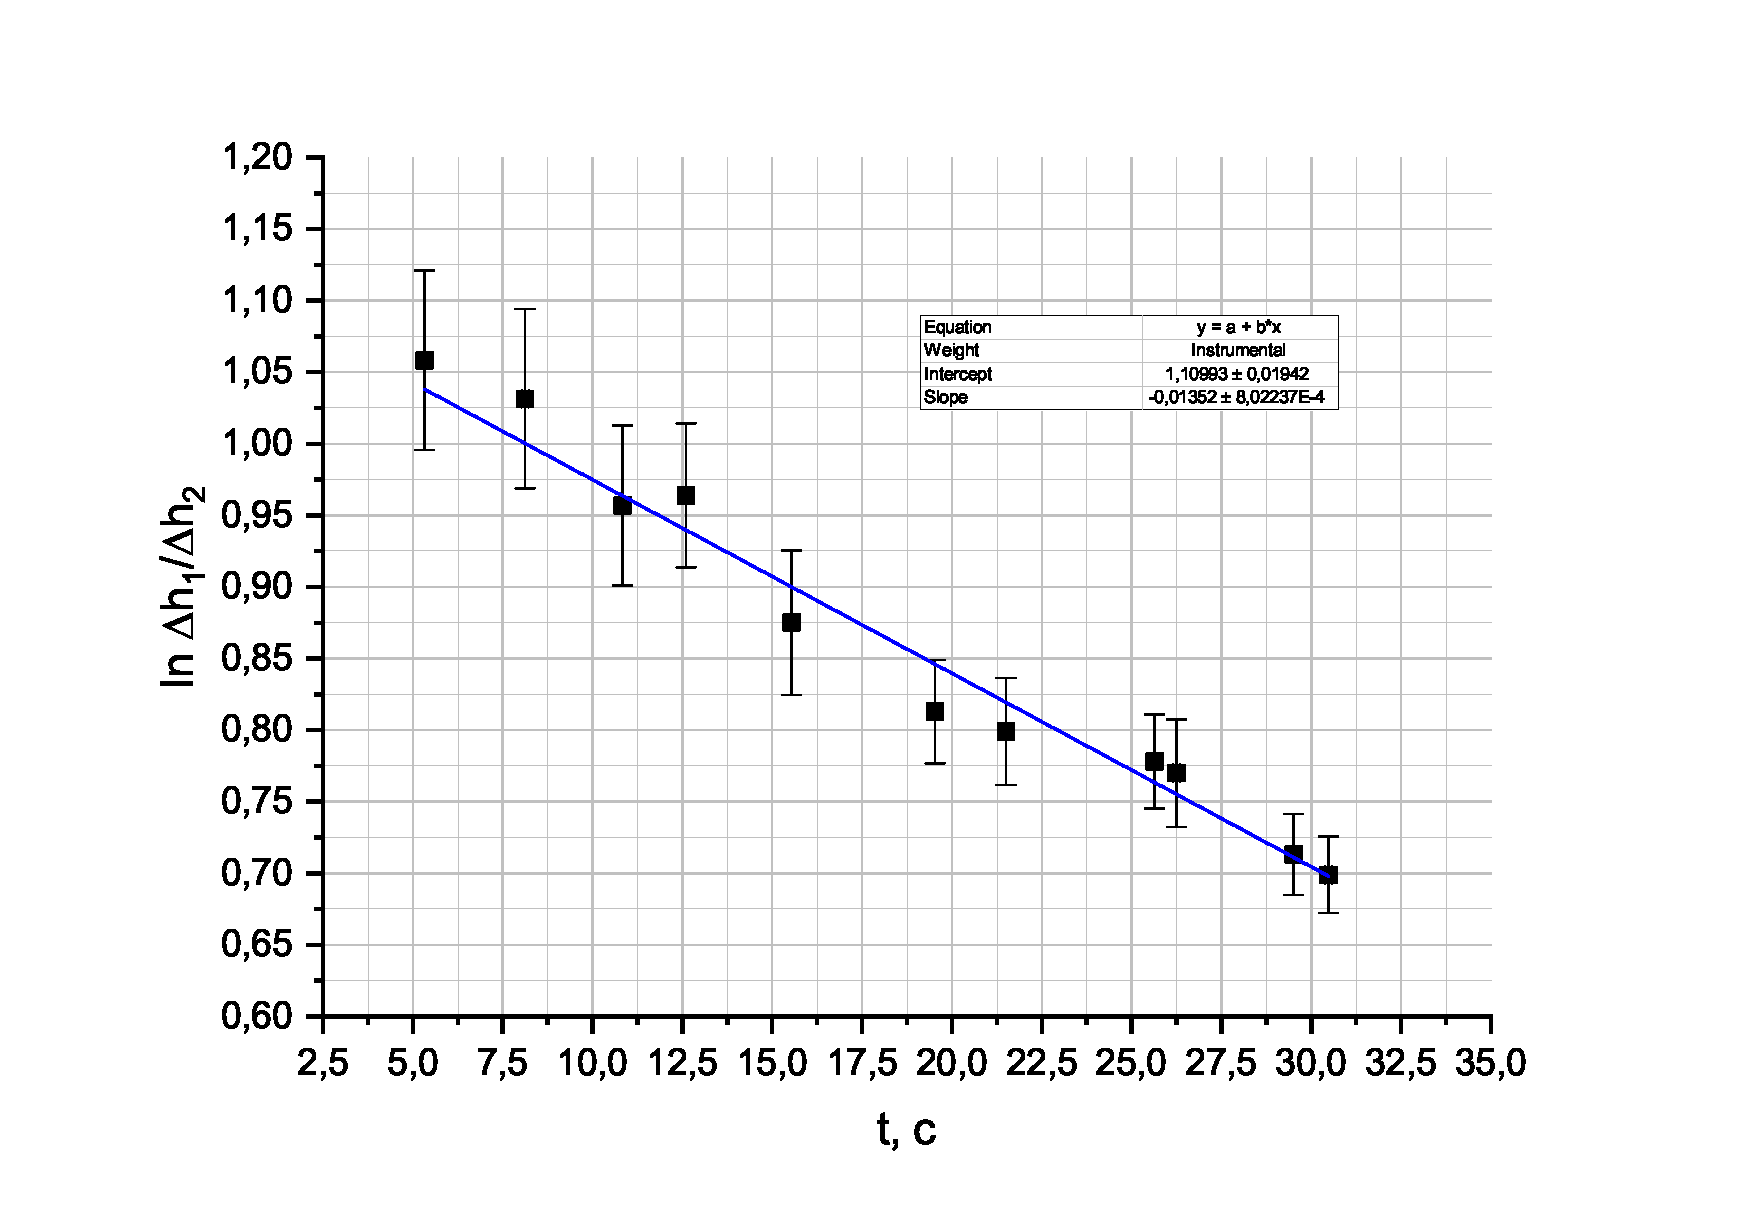
\includegraphics[width=\linewidth]{3}
	\end{center}
\end{figure}
\section{Обсуждение результатов и выводы}
В работе было проведено измерение показателя адиабаты для воздуха методом Клемана-Дезорма:
\[\gamma = 1,491\pm0,014\]
Также был детально исследован сам метод измерения. Были описаны условия, при которых необходимо проводить эксперимент и объяснено их влияние на результат.

Результаты получились немного завышены. В основном, это связано со временем открытия крана $\text{К}$ (Рис. 1)
\end{document}